\section{FinFET}\label{section:FinFET}

	\subsection{Technology Overview}
	  The Fin-shaped Field Effect Transistor (FinFET) represents a fundamental shift in semiconductor device architecture, evolving from traditional planar structures to a three-dimensional, multi-gate Metal-Oxide-Semiconductor Field-Effect Transistor (MOSFET). This technological transition was principally motivated by the need to overcome the persistent challenges associated with short-channel effects (SCEs) that emerged as conventional planar CMOS devices were scaled to smaller process nodes.
	  The FinFET's unique structure, which features a vertical ``fin'' that serves as the channel, provides superior electrostatic control compared to its planar predecessors. The operation of the device is governed by key geometric parameters, as illustrated in Figure \ref{fig:FinFET:FinFet-Overview}. The width of the fin ($W_{\symup{Fin}}$) is the critical dimension that dictates the electrostatic integrity of the channel. Meanwhile, the height of the fin ($H_{\symup{Fin}}$) is the primary parameter that controls the drive current of the transistor.\par

	  \begin{figure}[h!]
			\centering
			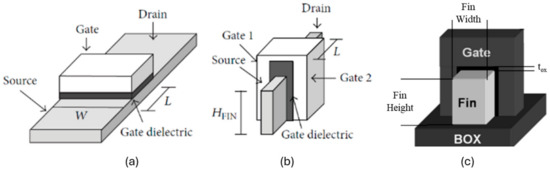
\includegraphics[scale=0.5]{assets/FinFET/FinFET-Overview.jpg}
			\caption{Structure Schematic of (a) planar MOSFET and (b) FinFET. (c) Demonstrating $H_{\symup{Fin}}$ as fin height and $W_{\symup{Fin}}$ as fin width. Taken from \cite{FinFET1}.}
			\label{fig:FinFET:FinFet-Overview}
		\end{figure}

	\subsection{Historical Development}

	To fully contextualize the introduction of FinFET technology, it is essential to review the key historical developments in semiconductor devices that preceded it. This progression illustrates the industry's response to escalating demands for miniaturization, speed, and power efficiency \cite{FinFET2}.\par

	The timeline of the modern electronics industry begins in 1904 with the launch of the vacuum tube \cite{FinFET2}. The vacuum tube, which controls the flow of electrons in a vacuum \cite{FinFET2}, served as the foundation of electronics for decades. However, it suffered from significant drawbacks, including diminished reliability, high power consumption, large physical size, and high manufacturing costs \cite{FinFET2}.\par

	The limitations of vacuum tubes led researchers to develop solid-state alternatives. A breakthrough occurred in 1947 with the construction of the point-contact transistor by William Shockley, John Bardeen, and Walter Brattain. This was followed in 1948 by William Shockley's invention of the Bipolar Junction Transistor (BJT) \cite{FinFET2}. These semiconductor devices proved to be far more reliable and power-efficient than vacuum tubes \cite{FinFET2}.\par

	A pivotal advancement in transistor technology occurred in 1956. During this period, M.M. Atalla addressed critical issues regarding semiconductor surfaces, identifying silicon dioxide as an effective solution for stabilization \cite{FinFET2}. This research led directly to the design of the Insulated-Gate Field Effect Transistor (IGFET), now universally known as the Metal-Oxide-Semiconductor Field-Effect Transistor (MOSFET) \cite{FinFET2}.\par

	The capacity for integration soon followed. In 1958, Jack Kilby developed the first integrated circuit (IC), which successfully joined several transistors on a single silicon substrate \cite{FinFET2}. The MOSFET proved exceptionally suitable for this high-density integration and became the driving engine of the digital world for over four decades \cite{FinFET2}.\par

	As device scaling continued, planar MOSFETs began to face significant challenges, such as short-channel effects. This necessitated a fundamental change in transistor architecture. This evolutionary path led to the fabrication of the first quasi-planar FinFET device in 2001 by N. Lindert et al., which was developed to suppress the DIBL (Drain-Induced Barrier Lowering) effect and enable further scaling \cite{FinFET2}.\par

	\subsection{FinFET Classifications}
	FinFET technology is not monolithic; rather, it encompasses several structural variations. These devices can be categorized based on three primary aspects: the substrate used, the gate terminal configuration, and the geometry of the dielectric.\break

	\subsubsection{Classification by Substrate}
	The first classification distinguishes FinFETs based on their fundamental physical structure and substrate. Bulk FinFETs, as illustrated in Figure \ref{fig:FinFET:class-substrate}(a) from the source material, are fabricated on a standard silicon substrate \cite{FinFET1}. In this configuration, the individual fins share a common substrate and are physically connected \cite{FinFET1}. This structure closely resembles that of traditional planar MOSFETs, which simplifies the manufacturing transition and integration process, leading many companies to prefer this approach \cite{FinFET1}. SOI (Silicon-on-Insulator) FinFETs, as Shown in Figure \ref{fig:FinFET:class-substrate}(b), are designed with physically isolated fins that sit atop a Buried Oxide (BOX) layer \cite{FinFET1}. This isolation from the silicon substrate provides distinct operational features \cite{FinFET1}. The choice between Bulk and SOI structures involves a complex engineering trade-off based on factors such as fabrication cost and specific performance requirements \cite{FinFET1}.

	\begin{figure}[h!]
			\centering
			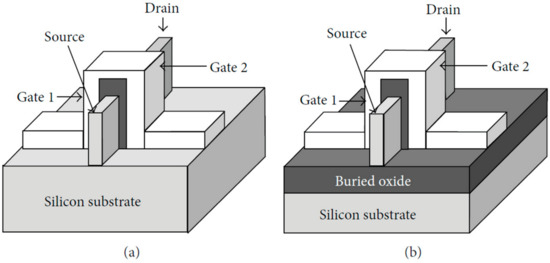
\includegraphics[scale=0.5]{assets/FinFET/fet-class-substrate.jpg}
			\caption{Structure schematic of (a) Bulk FinFET and (b) SOI FinFET \cite{FinFET1}.}
			\label{fig:FinFET:class-substrate}
	\end{figure}

	\subsubsection{Classification by Gate Type}
	The second classification is based on the number of terminals and the configuration of the gates, as shown in Figure \ref{fig:FinFET:class-gate} \cite{FinFET1}.
	Short Gate (SG) FinFETs are three-terminal devices where the two gates (Gate 1 and Gate 2) are physically connected, or "shorted," to each other \cite{FinFET1}. Independent Gate (IG) FinFETs are four-terminal devices. In this structure, the gates are physically isolated from one another by a dielectric material \cite{FinFET1}. This isolation allows for greater versatility, as varying voltages and signals can be applied to each gate terminal independently \cite{FinFET1}. IG FETs offer a superior $\nicefrac{I_{\symup{on}}}{I_{\symup{off}}}$ ratio because the voltage of one gate can be adjusted by the other, making them particularly well-suited for power management applications \cite{FinFET1}.

	\begin{figure}[h!]
		\centering
		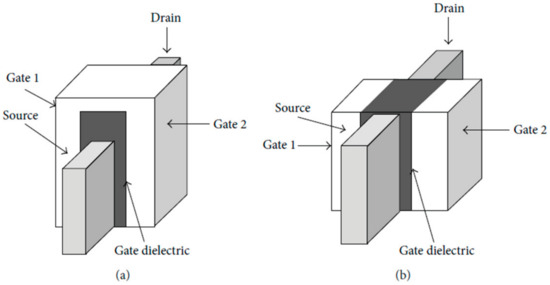
\includegraphics[scale=0.5]{assets/FinFET/fet-class-gate_type.jpg}
		\caption{Structure schematic of (a) SG FinFET and (b) IG FinFET. Taken from \cite{FinFET1}.}
		\label{fig:FinFET:class-gate}
	\end{figure}

	\subsubsection{Classification by Dielectric Geometry}
	The third classification, detailed in Figure \ref{fig:FinFET:class-dielectric} of the source, differentiates devices by the gate's coverage of the fin, which is determined by the dielectric thickness and geometry \cite{FinFET1}. In Double-Gate (DG) FinFET structure, a hard mask is employed on top of the fin. This effectively results in two gates, one on each vertical sidewall, with the top surface being non-conductive. The effective channel width is therefore calculated as two times the fin height \cite{FinFET1}. In a Tri-Gate FinFET configuration, the dielectric thickness on top of the fin is reduced, allowing the gate electrode to wrap over the top surface in addition to the two sidewalls \cite{FinFET1}. This creates a third gate, which enhances electrostatic control \cite{FinFET1}. Consequently, the total effective channel width for a Tri-Gate device is calculated as $(2 \times \text{fin height}) + \text{fin width}$ \cite{FinFET1}. This design offers distinct advantages, including lower gate-to-source capacitance and overall better performance, while maintaining strong electrostatic integrity \cite{FinFET1}.

	\begin{figure}[h!]
		\centering
		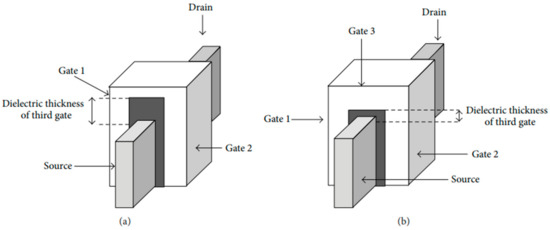
\includegraphics[scale=0.5]{assets/FinFET/fet-class-dielectric_geometry.jpg}
		\caption{Schematic of (a) DG FinFET and (b) tri-gate FinFET. Taken from \cite{FinFET1}.}
		\label{fig:FinFET:class-dielectric}
	\end{figure}

	\subsection{Materials in FinFET Fabrication}
	The performance, efficiency, and scalability of FinFET devices are critically dependent on the materials selected for their fabrication. Significant research has been directed toward optimizing materials for two key components: the gate dielectric and the channel.\par

	\subsubsection{Gate Dielectric Materials}
	A primary challenge in transistor scaling is the increase in gate leakage current as the traditional silicon dioxide ($\symup{SiO_2}$) dielectric layer becomes physically too thin \cite{FinFET1}. To counteract this, the industry has transitioned to high-k dielectric materials, which allow for a physically thicker layer while maintaining the same equivalent oxide thickness (EOT), thereby reducing leakage current \cite{FinFET1}. Hafnium Oxide ($\symup{HfO_2}$), for example, is a widely adopted high-k dielectric. Studies show that using $\symup{HfO_2}$ in a double-gate n-FinFET structure effectively reduces leakage current and offers significantly lower leakage than $\symup{SiO_2}$ \cite{FinFET1}.\par

	An even more cutting-edge high-k material is Lanthanum Zirconium Oxide ($\symup{LaZrO_2}$), which has a dielectric constant (k) of approximately 40, compared to 3.9 for $\symup{SiO_2}$ \cite{FinFET1}. As detailed in Table \ref{tab:gate-dielectrics}, its impact on device efficiency is substantial \cite{FinFET1}. When compared to $\symup{SiO_2}$ in an n-FinFET, $\symup{LaZrO_2}$ demonstrates a higher on-current ($I_{\symup{ON}}$) of $4.95 \times 10^{-5}$ A (versus $1.78 \times 10^{-5}$ A), a significantly lower off-current ($I_{\symup{OFF}}$) of $3.61 \times 10^{-14}$ A (versus $5.02 \times 10^{-13}$ A), and a dramatically improved $I_{\symup{ON}}/I_{\symup{OFF}}$ ratio of $1.37 \times 10^{9}$ (versus $3.50 \times 10^{7}$) \cite{FinFET1}. Furthermore, the $\symup{LaZrO_2}$ device shows a steeper Subthreshold Swing (SS) of 60.3 mV/dec and a much-reduced Drain-Induced Barrier Lowering (DIBL) effect of 10.1 mV/V, compared to 67.02 mV/dec and 43 mV/V for $\symup{SiO_2}$, respectively \cite{FinFET1}. These data confirm that high-k dielectrics are essential for enhancing electrostatic control, boosting the $I_{\symup{ON}}$/$I_{\symup{OFF}}$ ratio, and mitigating short-channel effects \cite{FinFET1}.\par

	\begin{table*}[]
	\centering
	\begin{tabular}{lll}
		\hline
		Parameters ($V_{\symup{d}}=0.75\unit{\volt}$, $V_{\symup{g}}=0.75\unit{\volt}$) & ($\symup{LaZrO}_{\symup{2}}$) Gate dielectric material $k = 40$ & ($\symup{SiO}_{\symup{2}}$) Gate dielectric material $k = 3.9$ \\
		\hline \hline
		$I_{\symup{ON}} (\unit{\ampere})$                            & $4.95 \times 10^{-5}$        & $1.78 \times 10^{-5}$        \\
		$I_{\symup{OFF}} (\unit{\ampere})$                           & $3.61 \times 10^{-14}$       & $5.02 \times 10^{-13}$       \\
		$\displaystyle\nicefrac{I_{\symup{ON}}}{I_{\symup{OFF}}}$    & $1.37 \times 10^{9}$         & $3.50 \times 10^{7}$         \\
		$V_{\symup{t}} (\unit{\volt})$                               & $0.253$                      & $0.207$                      \\
		SS $(\unit{{\milli\volt}\per{\decade}})$                     & $60.3$                       & $67.02$                      \\
		DIBL $(\unit{{\milli\volt}\per{\decade}})$                   & $10.1$                       & $43$                         \\
		\hline
	\end{tabular}
	\caption{The impact of $\symup{SiO_2}$ and $\symup{LaZrO_2}$ gate dielectric material usage in n-FinFET device efficiency.}
	\label{tab:gate-dielectrics}
\end{table*}

% For unit typesetting check https://www.tug.org/docs/latex/siunitx/siunitx.pdf

	\subsubsection{Channel Materials}
	In addition to dielectrics, optimization of the channel material is crucial. While silicon (Si) remains the dominant channel material, research into alternative materials has identified several candidates with superior properties for specific applications. For instance, in comparative simulations of SOI FinFET devices, 3C-SiC (Silicon Carbide) was found to exhibit the maximum $\nicefrac{I_{\symup{ON}}}{I_{\symup{OFF}}}$ ratio, calculated at $1.90 \times 10^{11}$, and the minimum $I_{\symup{OFF}}$ current, at $7.00 \times 10^{-19}\unit{\ampere}$ \cite{FinFET1}. Other materials, such as GaN (Gallium Nitride) and GaAs (Gallium Arsenide), are recognized for demonstrating superior DIBL characteristics, indicating better control over short-channel effects \cite{FinFET1}. Conversely, GaSb (Gallium Antimonide) has been identified as a poor-performing channel material, exhibiting the worst characteristics related to short-channel effects \cite{FinFET1}\par

	Looking forward, novel materials like Carbon Nanotubes (CNT) and Graphene are being investigated for their potential to significantly improve the $\nicefrac{I_{\symup{ON}}}{I_{\symup{OFF}}}$ ratio, increase operational speed, and reduce overall energy consumption in future FinFET devices \cite{FinFET1}. These material optimizations are part of a broad effort that also includes innovations like dual KK-structures for improving frequency response \cite{FinFET1}, InGaAs-on-Insulator for optimizing the on/off trade-off \cite{FinFET1}, and the use of Atomic Layer Deposition (ALD) for threshold voltage improvements \cite{FinFET1}.\par

	\subsection{Key Challenges in FinFET Technology}

	Despite their advantages over planar MOSFETs, the transition to FinFET technology introduces a unique set of fabrication and operational challenges. These must be addressed to optimize device performance and reliability.\par

	\subsubsection{Parasitic Capacitances}
	The three-dimensional nature of the FinFET, specifically the increased overlap region between the front and back gates, results in a higher incidence of parasitic capacitances compared to planar devices \cite{FinFET1}. As illustrated in Figure \ref{fig:FinFET:challenge-parasitic}, these capacitances exist between various terminals, such as gate-to-source/drain contacts (C2) and gate-to-source/drain diffusion (C3). This increased capacitance is a significant concern as it degrades the device's high-speed performance, leading to slower switching times \cite{FinFET1}.\par

	\begin{figure}[h!]
		\centering
		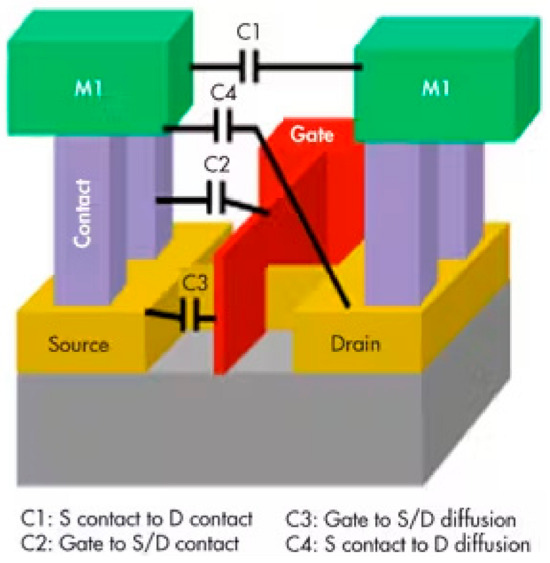
\includegraphics[width=0.5\linewidth]{assets/FinFET/fet-parasitic.jpg}
		\caption{Parasitic capacitances of a FinFET. Taken from \cite{FinFET1}.}
		\label{fig:FinFET:challenge-parasitic}
	\end{figure}

	\subsubsection{Corner Effects}
	A phenomenon unique to FinFETs is the ``corner effect''. While decreasing the fin width is effective for reducing short-channel effects, it can lead to a higher concentration of sub-threshold leakage current at the corners of the fin \cite{FinFET1}. This is due to enhanced electric fields at sharp edges \cite{FinFET1}. To mitigate this leakage path, FinFET production processes are modified to create fins with a more curved and rounded profile, as shown in the cross-sectional view in Figure \ref{fig:FinFET:challenge-corner} \cite{FinFET1}.\par

	\begin{figure}[h!]
		\centering
		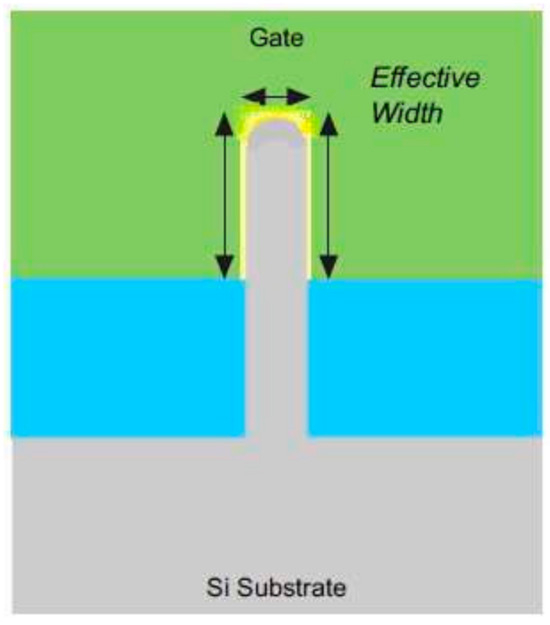
\includegraphics[width=0.5\linewidth]{assets/FinFET/fet-corner_effects.jpg}
		\caption{Cross-sectional view of a Tri-FinFET with curved fin corners. Taken from \cite{FinFET1}.}
		\label{fig:FinFET:challenge-corner}
	\end{figure}

	\subsubsection{Quantum Effects}\par
	As FinFETs scale to extremely thin fin widths, quantum mechanical effects become a significant performance limiter. In an ultra-thin fin, the density of available electron or hole states at the band edges diminishes \cite{FinFET1}. This ``quantum effect'' means that carriers (electrons or holes) require more energy to occupy states higher than the band edge before they can be liberated to conduct current \cite{FinFET1}. The practical result is a degradation of carrier mobility, which in turn reduces the drive current of the device.\par

	\subsubsection{Fabrication and Thermal Challenges}\par
	The fabrication of FinFETs is considerably more complex than that of planar MOSFETs. Creating the precise patterns for fins and gates demands an intricate level of process control, particularly in lithography \cite{FinFET1}. Furthermore, the narrow, tall structure of the fins poses thermal challenges. The smaller fin width, while beneficial for electrostatics, impedes the easy flow of heat out of the device, leading to an increase in device temperature \cite{FinFET1}. This phenomenon, known as self-heating, can negatively impact device reliability and performance.\par

	\subsection{Recent Innovations}
	To address the inherent challenges of FinFET technology, several structural innovations have been proposed to enhance performance and mitigate undesirable effects.

	The Ground-Plane FinFET (GP-FinFET), depicted in Figure \ref{fig:FinFET:innovation-gp}, introduces ground planes under the source and drain regions \cite{FinFET1}. This design was proposed to reduce the electric field coupling between the source and drain, thereby effectively minimizing Drain-Induced Barrier Lowering (DIBL) \cite{FinFET1}.\par

	\begin{figure}[h!]
		\centering
		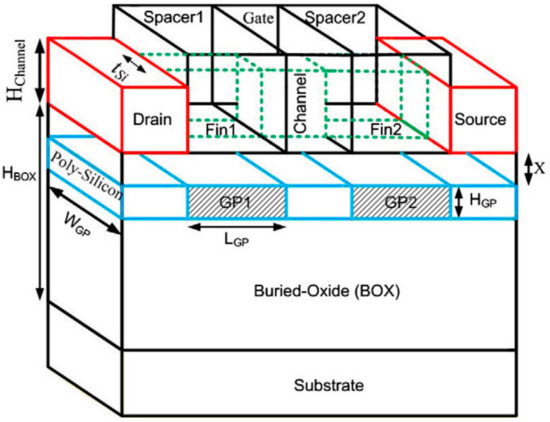
\includegraphics[width=0.6\linewidth]{assets/FinFET/finfet-gp.jpg}
		\caption{Three-dimensional view of the GP-FinFET structure schematic. Taken from \cite{FinFET1}.}
		\label{fig:FinFET:innovation-gp}
	\end{figure}

	A second innovation is the Bottom-Spacer (BS) FinFET, shown in Figure \ref{fig:FinFET:innovation-bs}. This structure was conceived to improve short-channel effect and self-heating performance \cite{FinFET1}. It incorporates an added spacer region that insulates the inactive (lower) portion of the fin from the gate contact, leading to improved control over short-channel effects and better thermal management \cite{FinFET1}.

	\begin{figure}[h!]
		\centering
		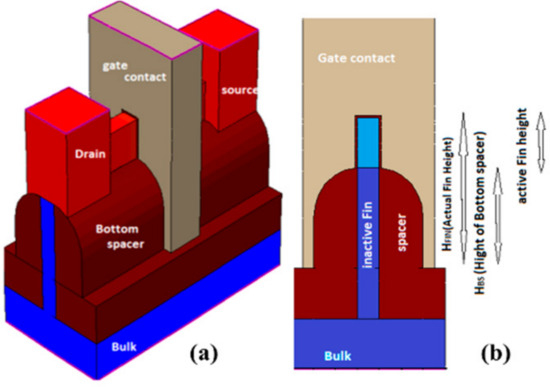
\includegraphics[width=0.7\linewidth]{assets/FinFET/finfet-bottom_spacer.jpg}
		\caption{(a) 3D view and (b) side view of the structure of bottom spacer FinFET. Taken from \cite{FinFET1}.}
		\label{fig:FinFET:innovation-bs}
	\end{figure}

	Finally, the Negative Capacitance FinFET with Ferroelectric Spacer (NCFS), illustrated in Figure \ref{fig:FinFET:innovation-ncfs}, employs a ferroelectric material in the spacer region rather than a traditional dielectric \cite{FinFET1}. The polarization of this ferroelectric material amplifies the electric field, which leads to enhancements in key performance metrics, including a higher on-state current ($I_{\symup{on}}$) and a lower, or steeper, subthreshold slope (SS) \cite{FinFET1}.

	\begin{figure}[h!]
		\centering
		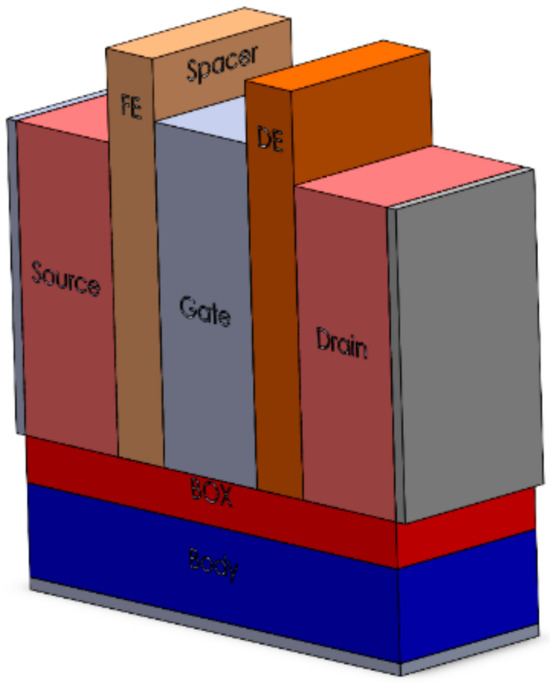
\includegraphics[width=0.45\linewidth]{assets/FinFET/finfet-negative_capacitance.jpg}
		\caption{Three-dimensional view of the most effective structure of Negative Capacitance FinFET with Ferroelectric Spacer. Taken from \cite{FinFET1}.}
		\label{fig:FinFET:innovation-ncfs}
	\end{figure}

	\subsection{Multi-Fin FinFET}

	A prevalent industry-standard implementation of the FinFET architecture is the Multi-Fin FinFET (M-FinFET). As illustrated in Figure \ref{fig:FinFET:n-finfet}, this design methodology positions multiple ``fins'', or channels, in parallel between the source and drain terminals \cite{FinFET2}.\par

	The primary advantage of this configuration is its ability to allow a higher number of charge carriers to traverse the device from source to drain simultaneously. This capability for increased current flow directly results in enhanced operational speed for the device \cite{FinFET2}.

	\begin{figure}[h!]
		\centering
		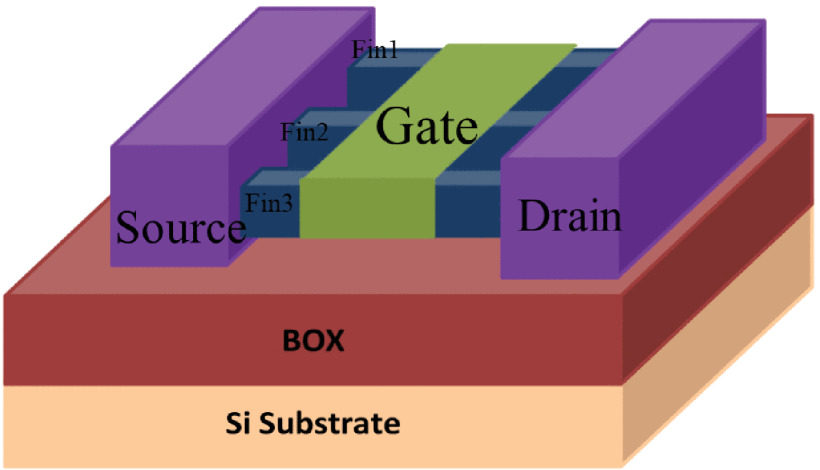
\includegraphics[scale=0.15]{assets/FinFET/m-finfet.jpg}
		\caption{Schematic diagram of M-FinFET. Taken from \cite{FinFET2}.}
		\label{fig:FinFET:n-finfet}
	\end{figure}

	\subsection{Motivation: Limitations of Planar MOSFETs}
	The development of FinFET technology was motivated by the fundamental limitations of traditional planar MOSFETs, as depicted in Figure \ref{fig:FinFET:mosfet}. As device scaling progressed to dimensions below $32\unit{\nano\meter}$, planar transistors began to exhibit significant performance issues \cite{FinFET2}.

	\begin{figure}[h!]
		\centering
		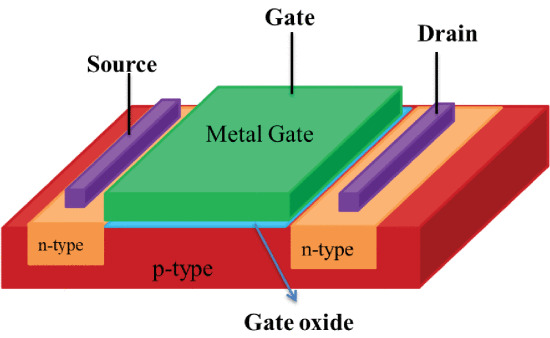
\includegraphics[scale=0.25]{assets/FinFET/planar-fet.jpg}
		\caption{The planar MOSFET semiconductor device. Taken from \cite{FinFET2}.}
		\label{fig:FinFET:mosfet}
	\end{figure}

	These issues include strong short-channel effects (SCE), a substantial increase in leakage currents, and greater threshold voltage variation \cite{FinFET2}. Such problems arise because the single gate of a planar device loses electrostatic control over the channel at small scales \cite{FinFET2}. This weak gate control leads to poor electrostatic integrity and significant power inefficiency.\par

	To overcome these scaling barriers, a new architecture was required\cite{FinFET2}. This necessitated the move to multi-gate structures (MuGFETs), such as the FinFET shown in Figure \ref{fig:FinFET:finfet-normal}, to re-establish strong gate control over the channel\cite{FinFET2}.

	\begin{figure}[h!]
		\centering
		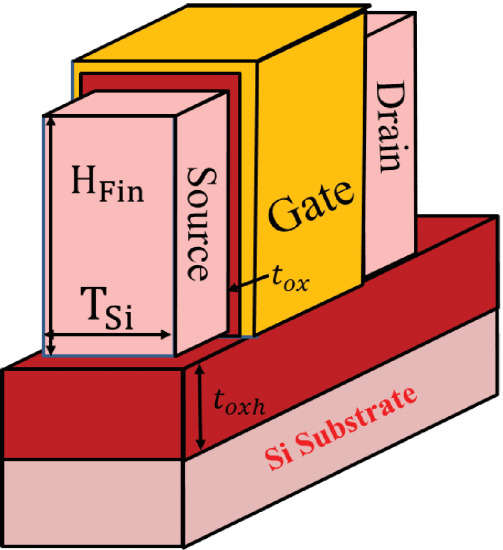
\includegraphics[scale=0.15]{assets/FinFET/fet-normal.jpg}
		\caption{Schematic diagram of conventional FinFET. Taken from \cite{FinFET2}.}
		\label{fig:FinFET:finfet-normal}
	\end{figure}


	\subsection{Conclusion: The Next Generation}

	FinFET technology has been instrumental in continuing semiconductor advancement, providing a scalable, low-power solution that has extended down to the $5\unit{\nano\meter}$ node \cite{FinFET1}. However, as FinFETs approach their physical scaling limits, they face persistent challenges in areas such as thermal management \cite{FinFET2} and manufacturing cost and complexity \cite{FinFET1}.\par

	To overcome these barriers and enable further miniaturization, the industry is transitioning to the next evolutionary architecture: the Gate-All-Around (GAA) FET \cite{FinFET2}. As illustrated in Figure \ref{fig:FinFET:fet-gaa}, the GAA structure offers superior electrostatic control by enveloping the channel from all sides, a critical requirement for nodes below $5\unit{\nano\meter}$.\par

	This transition from FinFET to GAA is not merely a future prospect; it is the industry's current trajectory. Samsung has been a pioneer in this shift, having introduced its first-generation $3\unit{\nano\meter}$ GAA MBCFET chips in 2022 \cite{FinFET2}\cite{FinFET3-samsung}. Meanwhile, Intel is introducing its GAA-based ``RibbonFET'' technology around 2026 \cite{FinFET4-intel}, and TSMC is de-veloping its $2\unit{\nano\meter}$ GAA platform for a target launch also around 2026 \cite{FinFET5-tsmc}. This clear industry-wide pivot confirms that the GAA architecture is succeeding the FinFET as the new standard to enable the future of semiconductor technology.

	\begin{figure}[h!]
		\centering
		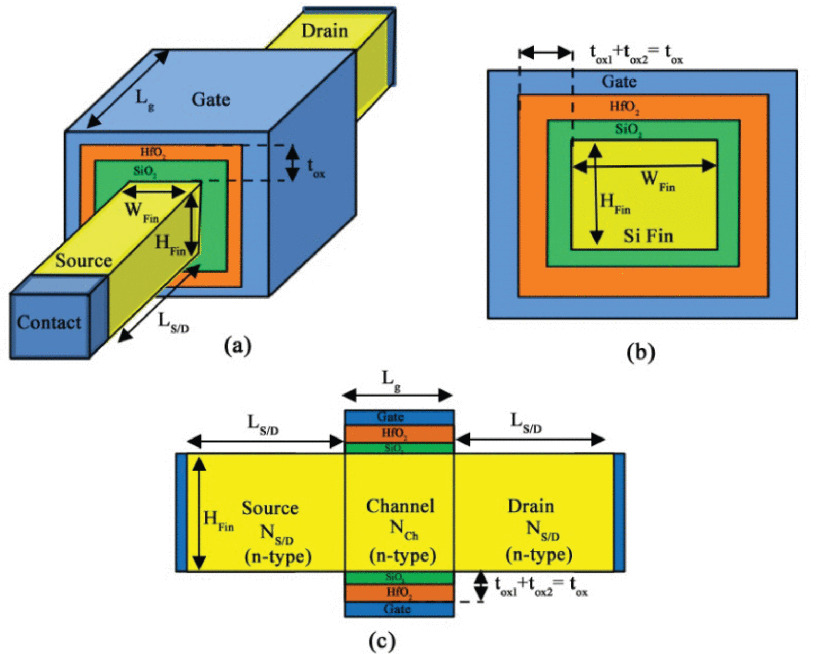
\includegraphics[width=0.75\linewidth]{assets/FinFET/GAA-FET.jpg}
		\caption{Schematic diagram of GAA structure along (a) Vertical (b) and horizontal view (c). Taken from \cite{FinFET2}.}
		\label{fig:FinFET:fet-gaa}
	\end{figure}
